% Benchmark study, started 2026-11-04.  Grows one benchmark and route at a time.
% Build:  python tools/benchmark_study/analyze.py && python tools/benchmark_study/report.py && tectonic main.tex
% Every table and figure in generated/ and figures/ is written by those scripts from the simulation records;
% only sections/*_findings.tex is written by hand, and every number in it is copied from the generated tables.
\documentclass[11pt,a4paper]{report}
\usepackage[margin=22mm]{geometry}
\usepackage[T1]{fontenc}
\usepackage{lmodern,booktabs,array,amsmath,xcolor,graphicx,float,caption,hyperref,enumitem}
\hypersetup{colorlinks=true,urlcolor=blue,linkcolor=black}
\captionsetup{font=small,labelfont=bf}
\setlength{\parindent}{0pt}\setlength{\parskip}{5pt}\setlength{\emergencystretch}{3em}
\setlist{itemsep=2pt,topsep=2pt}
\graphicspath{{figures/}}
\newcommand{\code}[1]{\texttt{\detokenize{#1}}}

\title{EPR pre-generation on ten benchmarks\\[3pt]\large ODG, CGP, ACGP and compiler-driven Dynamic, memories per core $K=1$ to $\infty$}
\author{BTP, MARS Lab, IIT Guwahati}
\date{Started 4 November 2026}

\begin{document}
\maketitle
\tableofcontents

\chapter{Setup}
\section{Architecture and workloads}
\begin{itemize}
\item $4\times4$ mesh of 16 cores; each core has 16 data slots, 14 occupied at the start and 2 kept free for migration,
      so circuits have $16\times14=224$ logical qubits.
\item Benchmarks: ten MQT Bench~2.3.0 circuits at 224 qubits (\code{benchmarks/}, verified by
      \code{benchmarks/verify.py}). Each is mapped once (T-HQA placer, OEE initial placement, mapping seed 42) and routed
      with XY and with history routing (history counts the route visits of all preceding layers, i.e.\ cumulative history, routing capacity 8); every strategy and every $K$ sees the same frozen trace.
\item Physics (\code{config/final_config/grid_4x4_ace_3.json}): memory efficiency 0.8, memory fidelity 0.95, coherence
      1\,s, detector efficiency 0.95. The classical delay is set by the topology code to about 0.1\,ms between neighbours.
\end{itemize}

\section{Strategies and policy}
ODG generates every pair on demand. CGP and ACGP generate pairs continuously into a cache. Dynamic is compiler driven:
the planner chooses, before the run, the layer in which each pair is started.
Everything except $K$ and the memory split is the default policy of the code (branch \code{history-algo-update},
\code{ace/compiler/settings.py}):
\begin{table}[H]\centering\small
\begin{tabular}{ll}\toprule
Setting & Value\\\midrule
Layer basis, lead, lookahead, age limit & active layers; 1, 2, 10 layers\\
Generation budget & 8 launches per core per active layer\\
Preparation priority & trace order (\code{trace})\\
Demand guard / refill on release & on / on\\
Admission & per-qubit, event driven, ready pairs first, longer chains first\\
Empty-layer gap & 10\,ns\\
Compiler reservation, pair use & 50\,ms, handoff\\
Physics seeds & 60 and 61\\\bottomrule
\end{tabular}
\caption{Default policy used in every run.}\end{table}

\section{Memories per core and the split}
\begin{table}[H]\centering\small
\begin{tabular}{lrrrrrrr}\toprule
$K$ (memories per core) & 1 & 2 & 3 & 4 & 6 & 8 & $\infty$ (64)\\\midrule
Dynamic may use & 1 & 2 & 3 & 4 & 6 & 6 & 64\\
CGP / ACGP cache ($\lfloor0.75K\rfloor$) & 0 & 1 & 2 & 3 & 4 & 6 & 48\\\bottomrule
\end{tabular}
\caption{Pre-generation share of the $K$ memories. At $K=8$ six memories are reserved for pre-generation. CGP/ACGP use
$\lfloor0.75K\rfloor$ because caching in all $K$ memories starves requests (smoke test: 150--1060\,ms per hop at
$K=1$--4); at $K=1$ they therefore equal ODG.}\end{table}

\section{Metrics}
A \emph{hop} is one request between neighbouring cores; a \emph{chain} is all hops of one qubit in one layer.
\begin{description}
\item[Latency] mean time per hop from eligibility to EPR delivery, including any wait for a free memory.
\item[Fidelity] mean fidelity of the delivered pairs (not a circuit fidelity).
\item[Coverage] share of hops that found a pair already made: generation phase under 0.35\,ms, i.e.\ only the
      reservation handshake. Same definition for every strategy. Chain full coverage: every hop of the chain ready.
\item[Utilisation] pairs used divided by pairs generated. \textbf{Wastage} $=100-$ utilisation: pairs that expired or
      were never used. ODG makes no pairs in advance, so both are not applicable to it.
\end{description}
Bars are the mean of the two seeds; whiskers span the two seeds.

\chapter{Results}
\section{QFT, XY routing}
11076 hops; seeds 60, 61; every run completed every hop and passed the physical audit (Checks sheet of the workbook).
\subsection{Headline: 8 memories per core, 6 for pre-generation}
ODG, CGP, ACGP and Dynamic~(8) use 8 memories per core, of which 6 may hold pre-generated pairs; Dynamic~($\infty$) uses 64, which no core ever fills.
\begin{table}[H]\centering\small
\begin{tabular}{lrrrrrrr}\toprule
Configuration & Latency (ms) & p95 (ms) & Fidelity & Hop cov. (\%) & Chain full (\%) & Wastage (\%) & Utilisation (\%)\\\midrule
ODG & 1.782 & 4.60 & 0.9498 & 0.0 & 0.0 & -- & --\\
CGP & 0.970 & 3.25 & 0.9424 & 77.9 & 60.1 & 4.24 & 95.8\\
ACGP & 0.976 & 3.30 & 0.9421 & 77.6 & 60.0 & 4.39 & 95.6\\
Dynamic (8) & 0.747 & 2.25 & 0.9439 & 76.8 & 64.5 & 1.23 & 98.8\\
Dynamic ($\infty$) & 0.616 & 1.65 & 0.9442 & 84.0 & 71.9 & 1.18 & 98.8\\
\bottomrule\end{tabular}
\caption{QFT, XY routing, 8 memories per core, 6 for pre-generation: mean of the seeds.}\end{table}
\begin{figure}[H]\centering
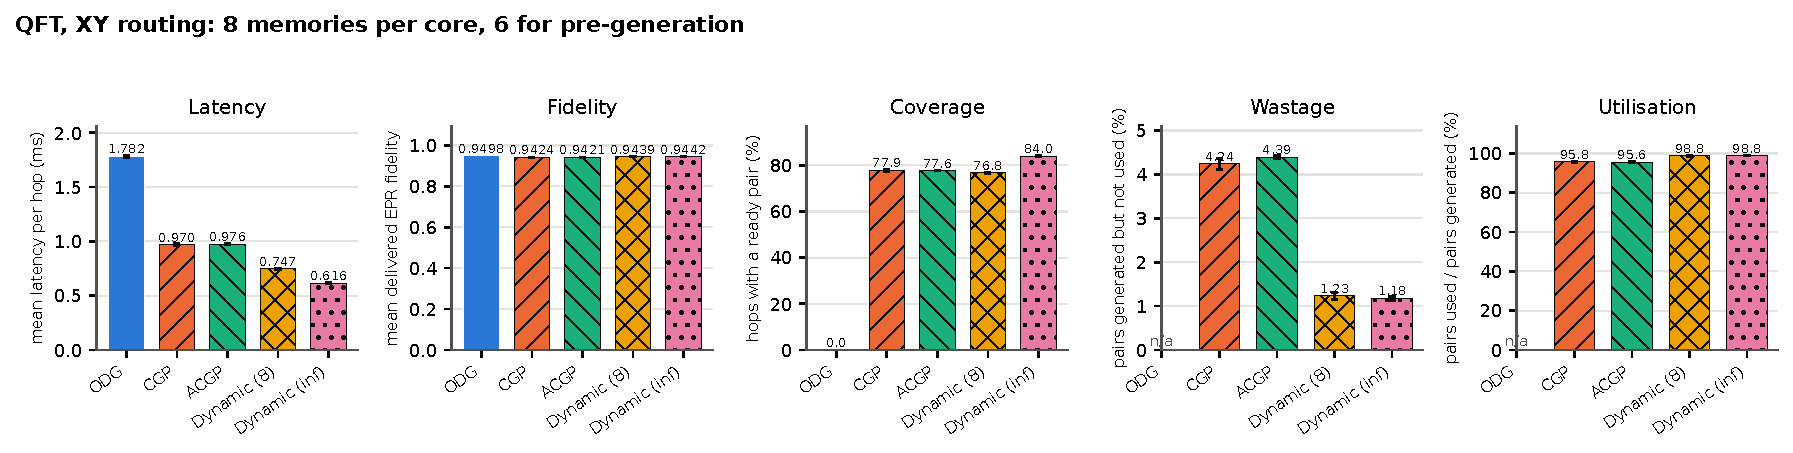
\includegraphics[width=\linewidth]{qft_xy_headline_8.pdf}
\caption{QFT, XY routing, 8 memories per core, 6 for pre-generation. Bars are the mean of the seeds, whiskers the seed range; fidelity bars start at zero, so read the labels.}\end{figure}
\subsection{Headline: 4 memories per core, all 4 for pre-generation}
ODG, CGP, ACGP and Dynamic~(4) use 4 memories per core and ODG and Dynamic may use all 4 for pre-generation; CGP and ACGP cache at most 3 (all 4 starves them), the same as in the $K$ sweep; Dynamic~($\infty$) as above.
\begin{table}[H]\centering\small
\begin{tabular}{lrrrrrrr}\toprule
Configuration & Latency (ms) & p95 (ms) & Fidelity & Hop cov. (\%) & Chain full (\%) & Wastage (\%) & Utilisation (\%)\\\midrule
ODG & 1.887 & 4.80 & 0.9498 & 0.0 & 0.0 & -- & --\\
CGP & 2.331 & 8.95 & 0.9401 & 63.0 & 41.7 & 5.87 & 94.1\\
ACGP & 2.325 & 8.95 & 0.9402 & 63.4 & 43.9 & 5.76 & 94.2\\
Dynamic (4) & 1.295 & 4.70 & 0.9425 & 63.7 & 54.1 & 3.89 & 96.1\\
Dynamic ($\infty$) & 0.616 & 1.65 & 0.9442 & 84.0 & 71.9 & 1.18 & 98.8\\
\bottomrule\end{tabular}
\caption{QFT, XY routing, 4 memories per core, all 4 for pre-generation: mean of the seeds.}\end{table}
\begin{figure}[H]\centering
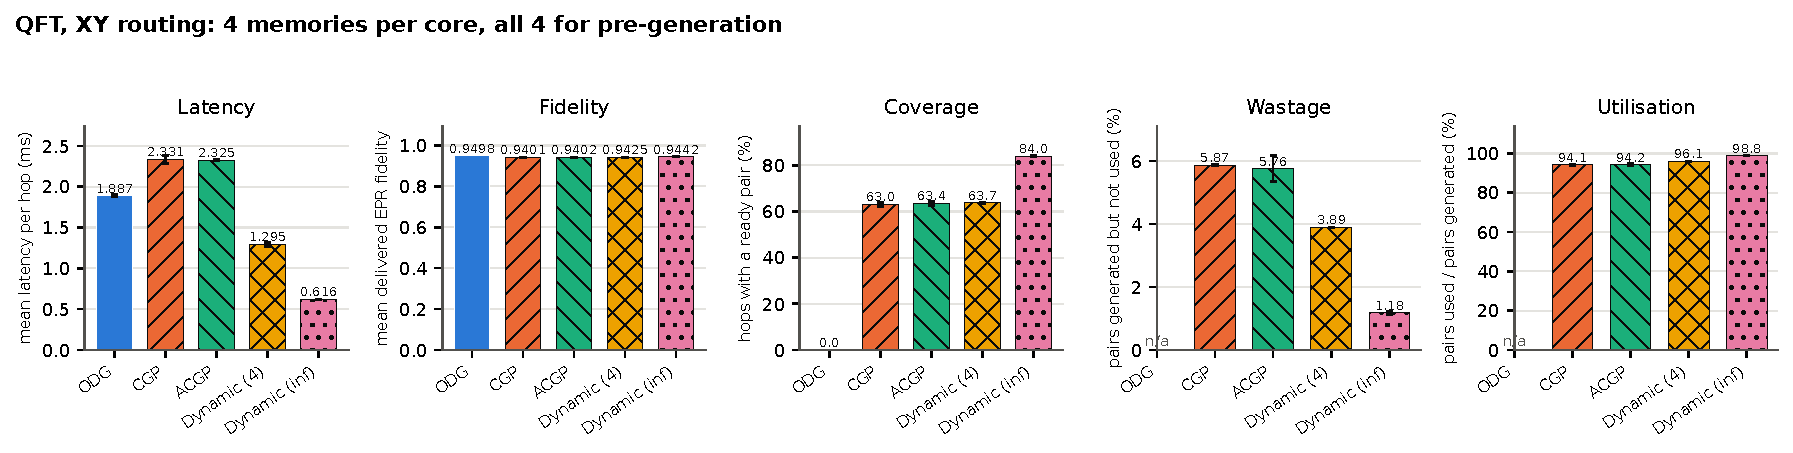
\includegraphics[width=\linewidth]{qft_xy_headline_4all.pdf}
\caption{QFT, XY routing, 4 memories per core, all 4 for pre-generation. Bars are the mean of the seeds, whiskers the seed range; fidelity bars start at zero, so read the labels.}\end{figure}
\subsection{Memories per core K}
Dynamic may use all K memories, except 6 of 8 at $K=8$; CGP and ACGP cache $\lfloor 0.75K\rfloor$ pairs (so at $K=1$ they are ODG). $K=\infty$ is 64 memories.
\begin{table}[H]\centering\small
\begin{tabular}{lrrrrrrr}\toprule
Latency & $K=1$ & $K=2$ & $K=3$ & $K=4$ & $K=6$ & $K=8$ & $K=\infty$\\\midrule
ODG & 6.275 & 2.816 & 2.109 & 1.887 & 1.788 & 1.782 & 1.782\\
CGP & 6.275 & 4.177 & 2.885 & 2.331 & 1.237 & 0.970 & 0.457\\
ACGP & 6.275 & 4.118 & 2.974 & 2.325 & 1.247 & 0.976 & 0.458\\
Dynamic & 9.041 & 3.528 & 1.877 & 1.295 & 0.866 & 0.747 & 0.616\\
\bottomrule\end{tabular}
\caption{QFT, XY routing: latency (mean latency per hop (ms)) for every K.}\end{table}
\begin{figure}[H]\centering
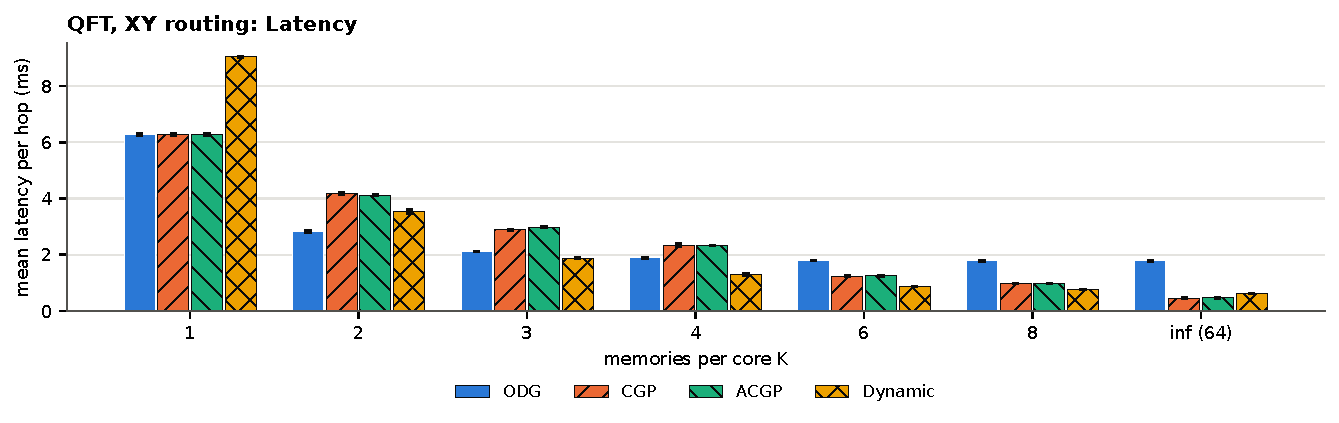
\includegraphics[width=\linewidth]{qft_xy_k_latency_ms.pdf}
\caption{QFT, XY routing: latency for every K.}\end{figure}
\begin{table}[H]\centering\small
\begin{tabular}{lrrrrrrr}\toprule
Fidelity & $K=1$ & $K=2$ & $K=3$ & $K=4$ & $K=6$ & $K=8$ & $K=\infty$\\\midrule
ODG & 0.9498 & 0.9498 & 0.9498 & 0.9498 & 0.9498 & 0.9498 & 0.9498\\
CGP & 0.9498 & 0.9441 & 0.9415 & 0.9401 & 0.9427 & 0.9424 & 0.9422\\
ACGP & 0.9498 & 0.9441 & 0.9414 & 0.9402 & 0.9425 & 0.9421 & 0.9422\\
Dynamic & 0.9486 & 0.9440 & 0.9429 & 0.9425 & 0.9432 & 0.9439 & 0.9442\\
\bottomrule\end{tabular}
\caption{QFT, XY routing: fidelity (mean delivered EPR fidelity) for every K.}\end{table}
\begin{figure}[H]\centering
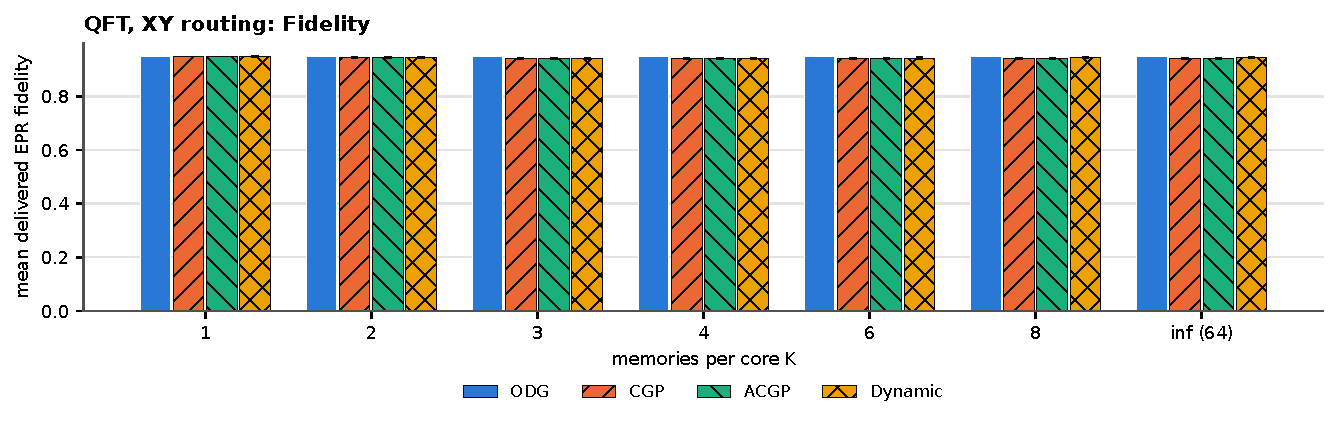
\includegraphics[width=\linewidth]{qft_xy_k_fidelity.pdf}
\caption{QFT, XY routing: fidelity for every K.}\end{figure}
\begin{table}[H]\centering\small
\begin{tabular}{lrrrrrrr}\toprule
Coverage & $K=1$ & $K=2$ & $K=3$ & $K=4$ & $K=6$ & $K=8$ & $K=\infty$\\\midrule
ODG & 0.0 & 0.0 & 0.0 & 0.0 & 0.0 & 0.0 & 0.0\\
CGP & 0.0 & 26.8 & 50.5 & 63.0 & 64.2 & 77.9 & 99.3\\
ACGP & 0.0 & 27.0 & 49.0 & 63.4 & 63.9 & 77.6 & 99.1\\
Dynamic & 8.9 & 36.3 & 52.4 & 63.7 & 76.8 & 76.8 & 84.0\\
\bottomrule\end{tabular}
\caption{QFT, XY routing: coverage (hops with a ready pair (\%)) for every K.}\end{table}
\begin{figure}[H]\centering
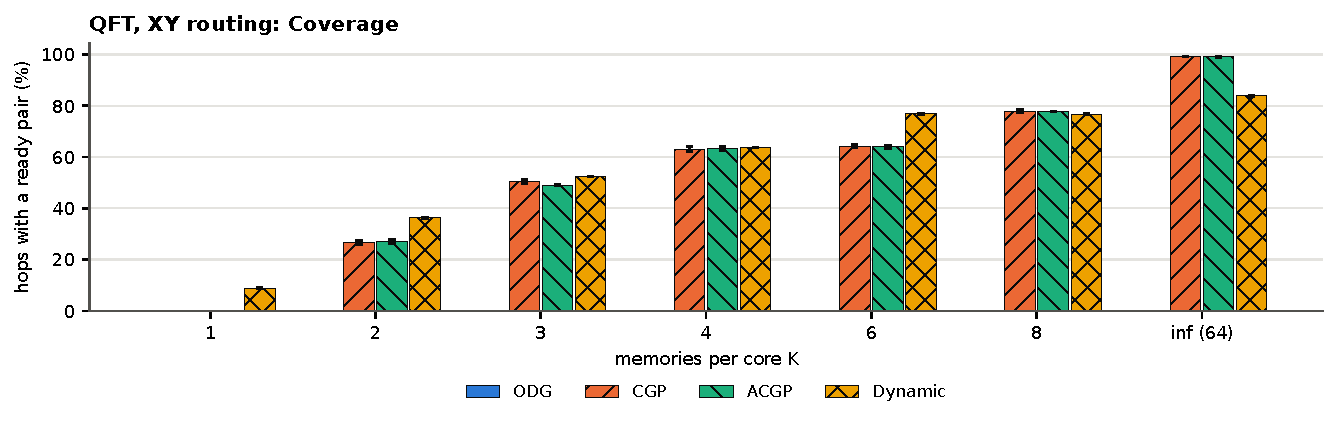
\includegraphics[width=\linewidth]{qft_xy_k_hop_coverage_pct.pdf}
\caption{QFT, XY routing: coverage for every K.}\end{figure}
\begin{table}[H]\centering\small
\begin{tabular}{lrrrrrrr}\toprule
Wastage & $K=1$ & $K=2$ & $K=3$ & $K=4$ & $K=6$ & $K=8$ & $K=\infty$\\\midrule
ODG & -- & -- & -- & -- & -- & -- & --\\
CGP & -- & 7.08 & 5.66 & 5.87 & 4.34 & 4.24 & 13.73\\
ACGP & -- & 7.04 & 6.13 & 5.76 & 4.49 & 4.39 & 13.73\\
Dynamic & 60.80 & 14.59 & 6.08 & 3.89 & 2.05 & 1.23 & 1.18\\
\bottomrule\end{tabular}
\caption{QFT, XY routing: wastage (pairs generated but not used (\%)) for every K.}\end{table}
\begin{figure}[H]\centering
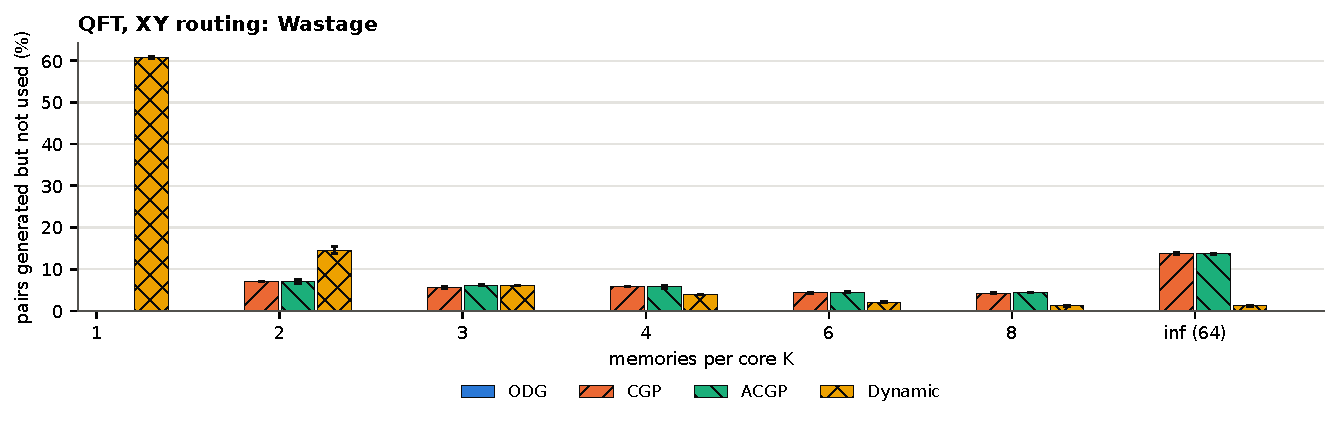
\includegraphics[width=\linewidth]{qft_xy_k_wastage_pct.pdf}
\caption{QFT, XY routing: wastage for every K.}\end{figure}
\begin{table}[H]\centering\small
\begin{tabular}{lrrrrrrr}\toprule
Utilisation & $K=1$ & $K=2$ & $K=3$ & $K=4$ & $K=6$ & $K=8$ & $K=\infty$\\\midrule
ODG & -- & -- & -- & -- & -- & -- & --\\
CGP & -- & 92.9 & 94.3 & 94.1 & 95.7 & 95.8 & 86.3\\
ACGP & -- & 93.0 & 93.9 & 94.2 & 95.5 & 95.6 & 86.3\\
Dynamic & 39.2 & 85.4 & 93.9 & 96.1 & 98.0 & 98.8 & 98.8\\
\bottomrule\end{tabular}
\caption{QFT, XY routing: utilisation (pairs used / pairs generated (\%)) for every K.}\end{table}
\begin{figure}[H]\centering
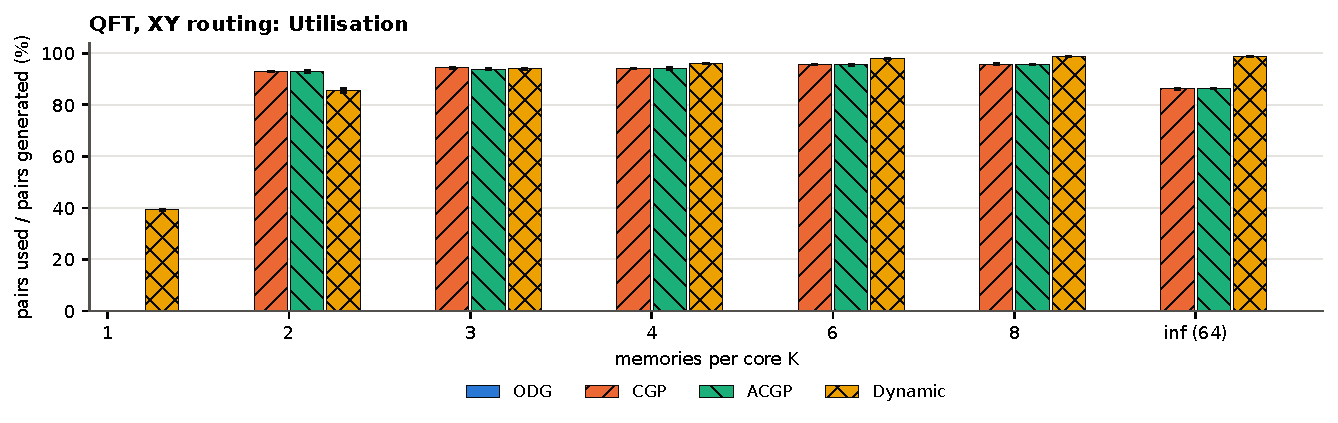
\includegraphics[width=\linewidth]{qft_xy_k_utilisation_pct.pdf}
\caption{QFT, XY routing: utilisation for every K.}\end{figure}

\clearpage
\section{QFT, history routing}
11076 hops; seeds 60, 61; every run completed every hop and passed the physical audit (Checks sheet of the workbook).
\subsection{Headline: 8 memories per core, 6 for pre-generation}
ODG, CGP, ACGP and Dynamic~(8) use 8 memories per core, of which 6 may hold pre-generated pairs; Dynamic~($\infty$) uses 64, which no core ever fills.
\begin{table}[H]\centering\small
\begin{tabular}{lrrrrrrr}\toprule
Configuration & Latency (ms) & p95 (ms) & Fidelity & Hop cov. (\%) & Chain full (\%) & Wastage (\%) & Utilisation (\%)\\\midrule
ODG & 1.773 & 4.40 & 0.9498 & 0.0 & 0.0 & -- & --\\
CGP & 0.966 & 3.10 & 0.9422 & 73.8 & 52.6 & 4.97 & 95.0\\
ACGP & 0.917 & 2.95 & 0.9425 & 76.6 & 57.4 & 4.34 & 95.7\\
Dynamic (8) & 0.693 & 2.00 & 0.9442 & 79.6 & 65.7 & 1.40 & 98.6\\
Dynamic ($\infty$) & 0.584 & 1.45 & 0.9450 & 85.6 & 72.4 & 1.46 & 98.5\\
\bottomrule\end{tabular}
\caption{QFT, history routing, 8 memories per core, 6 for pre-generation: mean of the seeds.}\end{table}
\begin{figure}[H]\centering
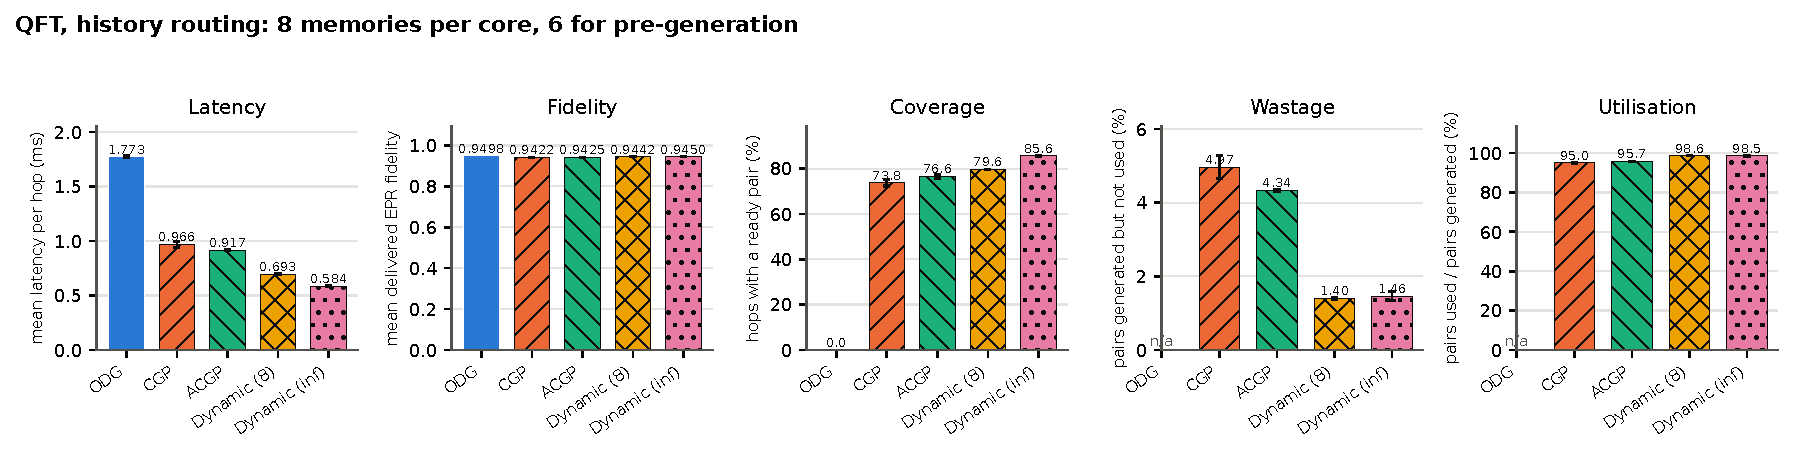
\includegraphics[width=\linewidth]{qft_history_headline_8.pdf}
\caption{QFT, history routing, 8 memories per core, 6 for pre-generation. Bars are the mean of the seeds, whiskers the seed range; fidelity bars start at zero, so read the labels.}\end{figure}
\subsection{Headline: 4 memories per core, all 4 for pre-generation}
ODG, CGP, ACGP and Dynamic~(4) use 4 memories per core and ODG and Dynamic may use all 4 for pre-generation; CGP and ACGP cache at most 3 (all 4 starves them), the same as in the $K$ sweep; Dynamic~($\infty$) as above.
\begin{table}[H]\centering\small
\begin{tabular}{lrrrrrrr}\toprule
Configuration & Latency (ms) & p95 (ms) & Fidelity & Hop cov. (\%) & Chain full (\%) & Wastage (\%) & Utilisation (\%)\\\midrule
ODG & 1.824 & 4.60 & 0.9498 & 0.0 & 0.0 & -- & --\\
CGP & 2.192 & 8.10 & 0.9413 & 63.5 & 40.3 & 5.37 & 94.6\\
ACGP & 2.194 & 8.14 & 0.9412 & 62.3 & 38.3 & 5.44 & 94.6\\
Dynamic (4) & 1.199 & 4.20 & 0.9423 & 65.8 & 55.5 & 4.45 & 95.6\\
Dynamic ($\infty$) & 0.584 & 1.45 & 0.9450 & 85.6 & 72.4 & 1.46 & 98.5\\
\bottomrule\end{tabular}
\caption{QFT, history routing, 4 memories per core, all 4 for pre-generation: mean of the seeds.}\end{table}
\begin{figure}[H]\centering
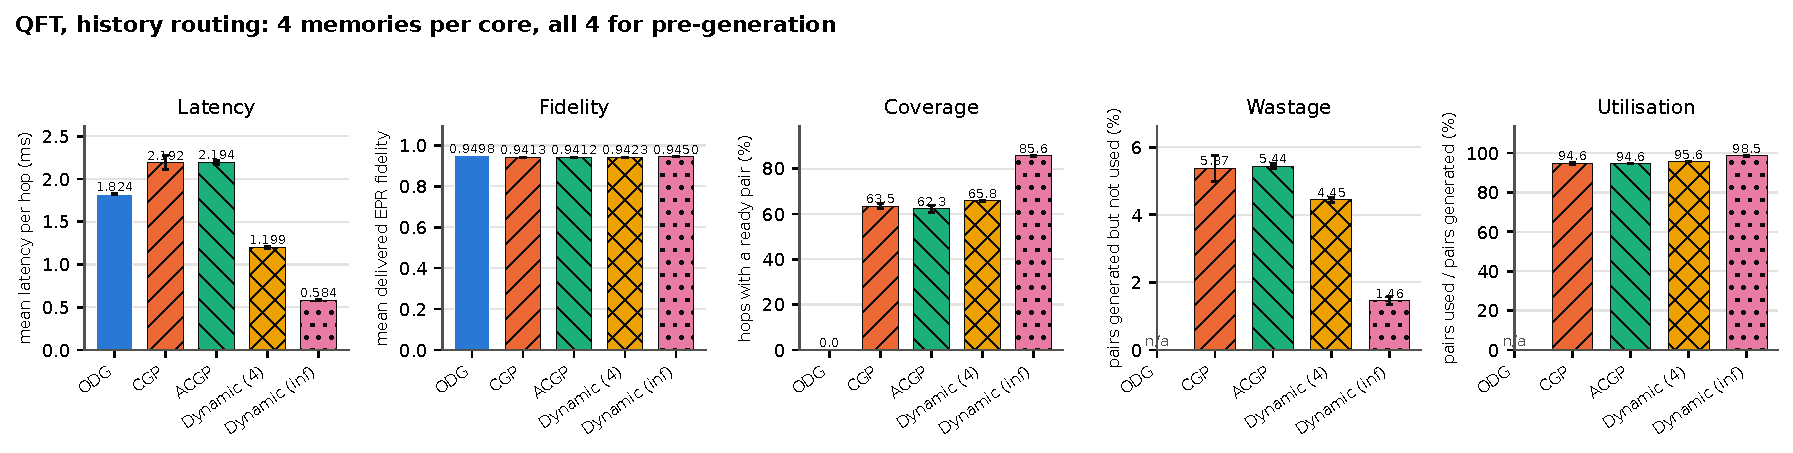
\includegraphics[width=\linewidth]{qft_history_headline_4all.pdf}
\caption{QFT, history routing, 4 memories per core, all 4 for pre-generation. Bars are the mean of the seeds, whiskers the seed range; fidelity bars start at zero, so read the labels.}\end{figure}
\subsection{Memories per core K}
Dynamic may use all K memories, except 6 of 8 at $K=8$; CGP and ACGP cache $\lfloor 0.75K\rfloor$ pairs (so at $K=1$ they are ODG). $K=\infty$ is 64 memories.
\begin{table}[H]\centering\small
\begin{tabular}{lrrrrrrr}\toprule
Latency & $K=1$ & $K=2$ & $K=3$ & $K=4$ & $K=6$ & $K=8$ & $K=\infty$\\\midrule
ODG & 5.820 & 2.554 & 1.963 & 1.824 & 1.776 & 1.773 & 1.773\\
CGP & 5.820 & 3.739 & 2.767 & 2.192 & 1.112 & 0.966 & 0.457\\
ACGP & 5.820 & 3.748 & 2.696 & 2.194 & 1.113 & 0.917 & 0.455\\
Dynamic & 8.812 & 3.153 & 1.749 & 1.199 & 0.797 & 0.693 & 0.584\\
\bottomrule\end{tabular}
\caption{QFT, history routing: latency (mean latency per hop (ms)) for every K.}\end{table}
\begin{figure}[H]\centering
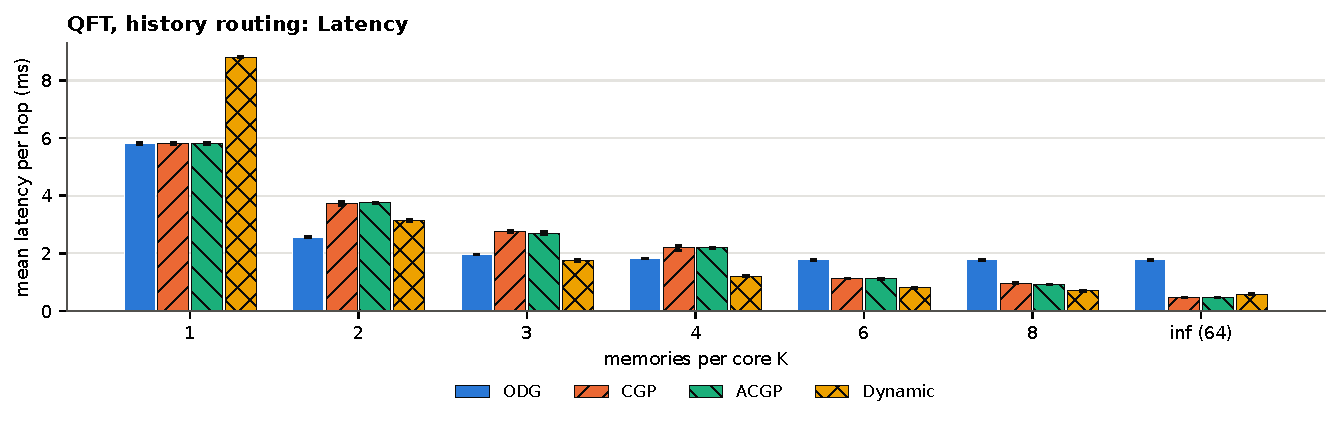
\includegraphics[width=\linewidth]{qft_history_k_latency_ms.pdf}
\caption{QFT, history routing: latency for every K.}\end{figure}
\begin{table}[H]\centering\small
\begin{tabular}{lrrrrrrr}\toprule
Fidelity & $K=1$ & $K=2$ & $K=3$ & $K=4$ & $K=6$ & $K=8$ & $K=\infty$\\\midrule
ODG & 0.9498 & 0.9498 & 0.9498 & 0.9498 & 0.9498 & 0.9498 & 0.9498\\
CGP & 0.9498 & 0.9452 & 0.9427 & 0.9413 & 0.9433 & 0.9422 & 0.9417\\
ACGP & 0.9498 & 0.9449 & 0.9426 & 0.9412 & 0.9433 & 0.9425 & 0.9418\\
Dynamic & 0.9487 & 0.9442 & 0.9427 & 0.9423 & 0.9439 & 0.9442 & 0.9450\\
\bottomrule\end{tabular}
\caption{QFT, history routing: fidelity (mean delivered EPR fidelity) for every K.}\end{table}
\begin{figure}[H]\centering
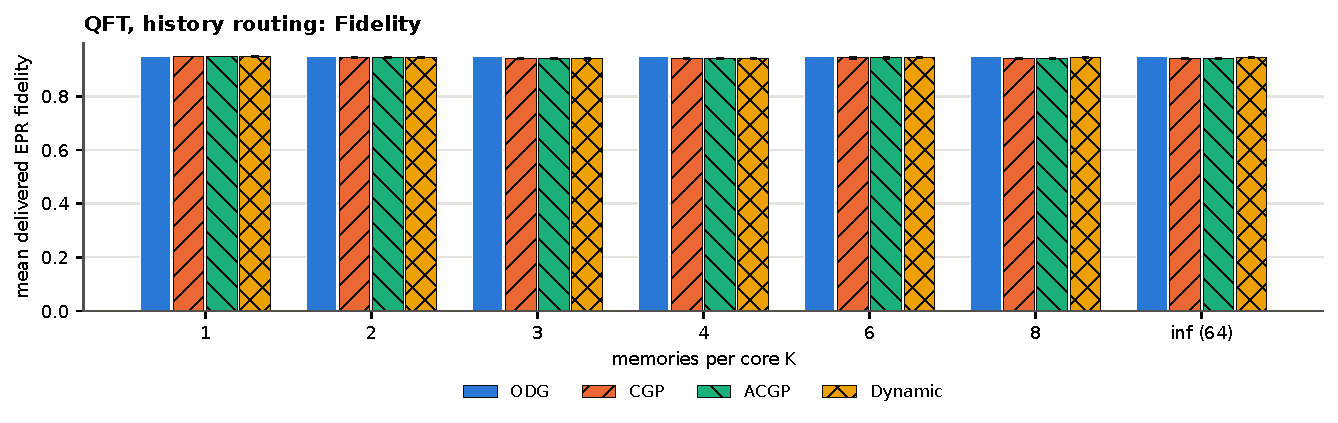
\includegraphics[width=\linewidth]{qft_history_k_fidelity.pdf}
\caption{QFT, history routing: fidelity for every K.}\end{figure}
\begin{table}[H]\centering\small
\begin{tabular}{lrrrrrrr}\toprule
Coverage & $K=1$ & $K=2$ & $K=3$ & $K=4$ & $K=6$ & $K=8$ & $K=\infty$\\\midrule
ODG & 0.0 & 0.0 & 0.0 & 0.0 & 0.0 & 0.0 & 0.0\\
CGP & 0.0 & 27.2 & 47.8 & 63.5 & 64.2 & 73.8 & 99.2\\
ACGP & 0.0 & 28.2 & 49.7 & 62.3 & 65.3 & 76.6 & 99.5\\
Dynamic & 8.4 & 36.4 & 53.8 & 65.8 & 79.2 & 79.6 & 85.6\\
\bottomrule\end{tabular}
\caption{QFT, history routing: coverage (hops with a ready pair (\%)) for every K.}\end{table}
\begin{figure}[H]\centering
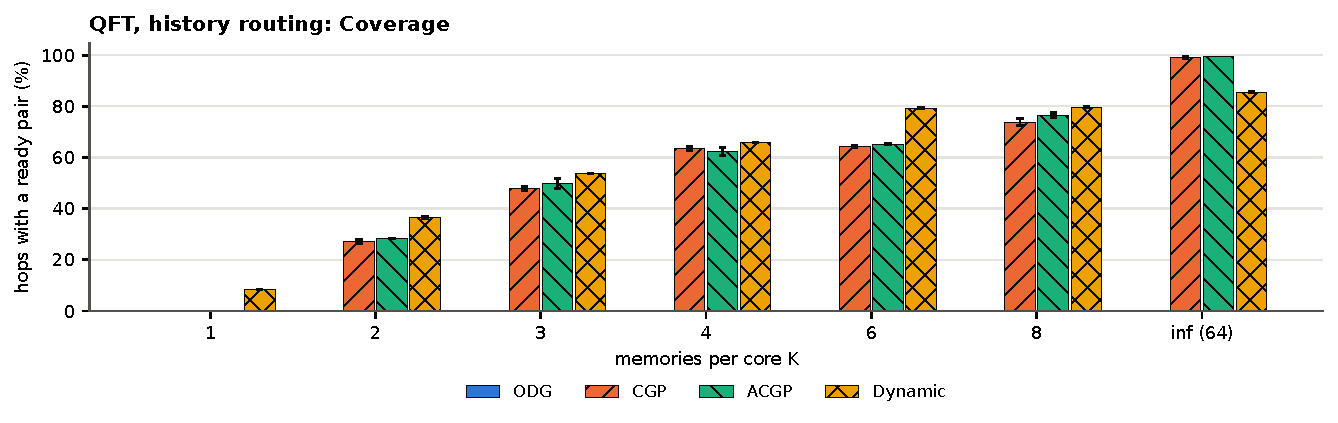
\includegraphics[width=\linewidth]{qft_history_k_hop_coverage_pct.pdf}
\caption{QFT, history routing: coverage for every K.}\end{figure}
\begin{table}[H]\centering\small
\begin{tabular}{lrrrrrrr}\toprule
Wastage & $K=1$ & $K=2$ & $K=3$ & $K=4$ & $K=6$ & $K=8$ & $K=\infty$\\\midrule
ODG & -- & -- & -- & -- & -- & -- & --\\
CGP & -- & 6.23 & 5.85 & 5.37 & 3.96 & 4.97 & 14.14\\
ACGP & -- & 6.07 & 5.58 & 5.44 & 3.74 & 4.34 & 13.66\\
Dynamic & 63.26 & 14.98 & 6.07 & 4.45 & 2.25 & 1.40 & 1.46\\
\bottomrule\end{tabular}
\caption{QFT, history routing: wastage (pairs generated but not used (\%)) for every K.}\end{table}
\begin{figure}[H]\centering
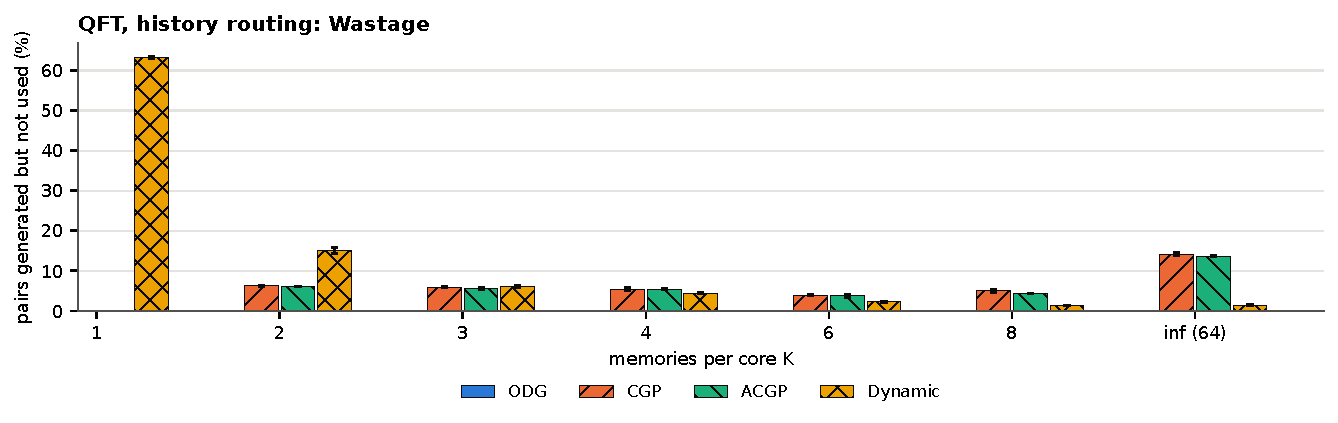
\includegraphics[width=\linewidth]{qft_history_k_wastage_pct.pdf}
\caption{QFT, history routing: wastage for every K.}\end{figure}
\begin{table}[H]\centering\small
\begin{tabular}{lrrrrrrr}\toprule
Utilisation & $K=1$ & $K=2$ & $K=3$ & $K=4$ & $K=6$ & $K=8$ & $K=\infty$\\\midrule
ODG & -- & -- & -- & -- & -- & -- & --\\
CGP & -- & 93.8 & 94.1 & 94.6 & 96.0 & 95.0 & 85.9\\
ACGP & -- & 93.9 & 94.4 & 94.6 & 96.3 & 95.7 & 86.3\\
Dynamic & 36.7 & 85.0 & 93.9 & 95.6 & 97.7 & 98.6 & 98.5\\
\bottomrule\end{tabular}
\caption{QFT, history routing: utilisation (pairs used / pairs generated (\%)) for every K.}\end{table}
\begin{figure}[H]\centering
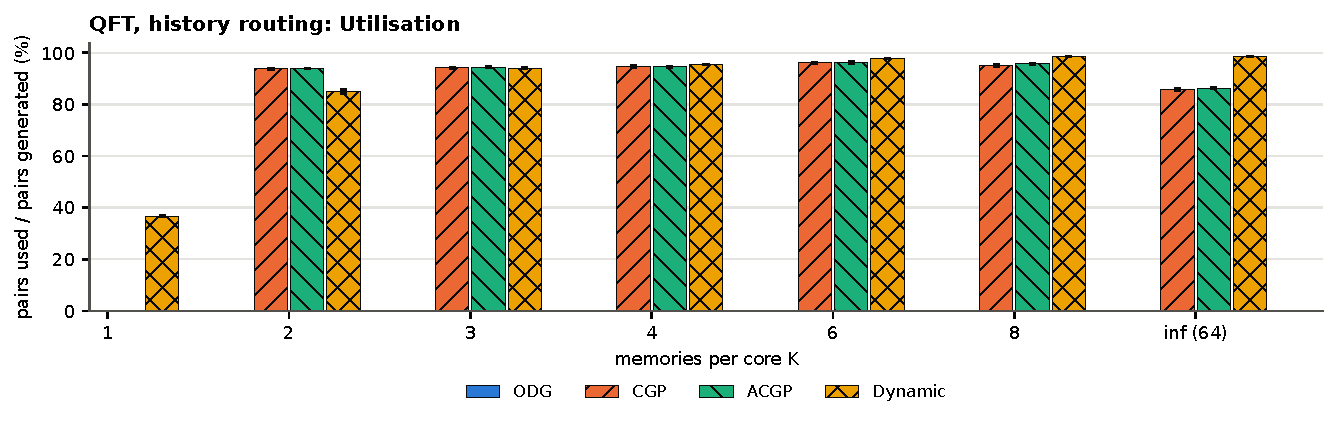
\includegraphics[width=\linewidth]{qft_history_k_utilisation_pct.pdf}
\caption{QFT, history routing: utilisation for every K.}\end{figure}

\clearpage


\end{document}
